
\section{Veje}
Vi har indtil videre snakket om punkter, og hvordan de som punktsæt forbindes med kanter. I dette afsnit vil vi udvide det til at snakke om veje, som er sekvenser af disse kanter. Hvis der er tale om ikke-orienterede grafer, er veje defineret ved:
\begin{defn}
[Veje] 
Lad $n$ være et ikke-negativt heltal og $G$ en ikke-orienteret graf. En vej af længde $n$ fra $u$ til $v$ i $G$ er en sekvens af n kanter $e_{1},e_{2},\cdots,e_{n}$ for $G$, for hvilket der eksisterer en sekvens $x_{0}=u,x_{1},x_{2},\cdots,x_{n-1}$,$x_{n}=v$ af punkter sådan at $e_{i}$ har, for $i=1,2,\cdots,n$, endepunkterne $x_{i-1}$ og $x_{i}$ Når grafen er simpel, betegner vi denne  vej ved dets punktsekvens $x_{o},x_{1},\cdots,x_{n}$ Vejen siges at passere igennem punkterne $x_{o},x_{1},\cdots,x_{n-1}$ eller krydse kanterne $e_{1},e_{2},\cdots,e_{n}$. En vej er simpel, hvis den ikke krydser den samme kant mere end én gang.
\end{defn}
Kigger vi derimod på veje med orienterede grafer, som er det vi beskæftiger os med i problemet, ser definitionen en smule anderledes ud:
\begin{defn}
[Veje] 
Lad $n$ være et ikke-negativt heltal og $G$ en orienteret graf. En vej af længde $n$ fra $u$ til $v$ i $G$ er en sekvens af kanter $e_{1},e_{2},\cdots,e_{n}$ for $G$, sådan at $e_{1}$ er forbundet med $(x_{0},x_{1})$, $e_{2}$ er forbundet med $(x_{1},x_{2})$ og så videre frem til $e_{n}$, som er forbundet med $(x_{n-1},x_{n})$. Her er $x_{0}=u$ og $x_{n}=v$. Hvis alle punktsæt er forbundet med højst én kant per sæt, betegner vi denne  vej ved dets punktsekvens $x_{o},x_{1},\cdots,x_{n}$. En vej er simpel, hvis den ikke krydser den samme kant mere end én gang.
\end{defn}

\begin{figure}[H]
\centering
	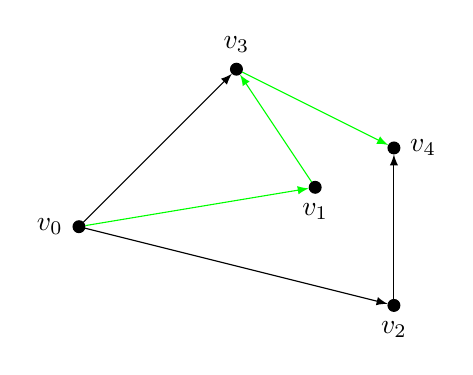
\begin{tikzpicture}

      \tikzset{enclosed/.style={draw, circle, inner sep=0pt, minimum size=.15cm, fill=black}}
%% Vertices
      	\node[enclosed, label={left: $v_0$}] (v0) at (0,2) {};
      	\node[enclosed, label={below: $v_1$}] (v1) at (3,2.5) {};
    		\node[enclosed, label={below: $v_2$}] (v2) at (4,1) {};
  	    \node[enclosed, label={above: $v_3$}] (v3) at (2,4) {};
     	\node[enclosed, label={right: $v_4$}] (v4) at (4,3) {};
%Edges
		\path [->, >=latex, green](v0) edge node[midway, sloped, above] {} (v1);
		\path [->, >=latex](v0) edge node[midway, sloped, above] {} (v2);
		\path [->, >=latex](v0) edge node[midway, above] {} (v3);
		\path [->, >=latex, green](v1) edge node[near end, sloped, below] {} (v3);
		\path [->, >=latex](v2) edge node[midway, below] {} (v4);
		\path [->, >=latex, green](v3) edge node[near end, sloped, above] {} (v4);

	\end{tikzpicture}
	\caption{Eksempel på en orienteret simpel graf og en vej fra $v_{0}$ til $v_{4}$}
	\label{fig.vaegtetopg}
\end{figure}


Antallet af veje mellem to punkter i grafen kan findes ved hjælp af nabomatricer, som vi diskuterede i forrige afsnit.
\begin{thm}
[Antallet af veje mellem to punkter] 
Lad G være en graf med nabomatricen
\textbf{$A$} med grafens punkter i rækkefølgen $v_{1},v_{2},\cdots,v_{n}$ (både orienterede og ikke-orienterede kanter samt flere kanter pr punktpar og løkker er tilladt). Antallet af forskellige veje med længde $r$ fra $v_{i}$ til $v_{j}$ vil da være lig den $(i,j)$'te indgang af \textbf{$A^{r}$}.
\end{thm}

\begin{proof}
Bevis: Lad G være en graf med nabomatricen 
\textbf{$A$}, hvor vi antager, at punkterne i $G$ har rækkefølgen $v_{1},v_{2},\cdots,v_{n}$. Antallet af veje fra $v_{i}$ til $v_{j}$ af længde 1 er da den $(i,j)$'te indagang til 
\textbf{$A$}. Dette skyldes, at det blot er antallet af kanter fra $v_{i}$ til $v_{j}$.
Vi antager at den $(i,j)$'te indagang til 
\textbf{${A^r}$} er antallet af forskellige veje som går fra $v_{i}$ til $v_{j}$ og som har længden $r$. Dette er hypotesen, vi ønsker at bekræfte.
Vi ser på nabomatricen \textbf{$A^{r+1}$}. 
\textbf{$A^{r+1}$} er det samme som 
\textbf{$A^{r}$}$\cdot$\textbf{$A$}, og derfor er den $(i,j)$'te indgang af \textbf{$A^{r+1}$} lig med $b_{i1}a_{1j} + b_{i2}a_{2j} +\cdots+ b_{in}a_{nj}$. Her er $b_{ik}$  den $(i,k)$'te indgang til 
\textbf{$A^{r}$}, som ifølge vores hypotese er antallet af veje fra $v_{i}$ til $v_{k}$ med længde $r$.
En vej af længde $r + 1$ fra $v_{i}$ til $v_{k}$ er lavet ud fra en vej med længden $r$ fra begyndelsespunktet $v_{i}$ og hen til et mellemliggende punkt $v_{k}$ samt den kant, der går fra $v_{k}$ til $v_{j}$. Vi ved fra kombinatorik at antallet af muligheder er lig prduktet af mulighederne ved første udfald og mulighederne ved andet udfald. Vi betegner antallet af veje med længden $r$ fra $v_{i}$ til $v_{k}$ med $b_{ik}$ og antallet af kanter fra $v_{k}$ til $v_{j}$ med $a_{kj}$ Finder vi produktet af dette for alle mellemliggende punkter, $v_{k}$, fås det ønskede resultat.
\end{proof}

\subsection{Eksempel}
Vi kan nu opstille et eksempel. Vi starter med at kigge på en graf og dens nabomatrix:
\begin{figure}[H]
\centering
	\begin{tikzpicture}

      \tikzset{enclosed/.style={draw, circle, inner sep=0pt, minimum size=.15cm, fill=black}}
%% Vertices
      	\node[enclosed, label={left: $v_0$}] (v0) at (1,2) {};
      	\node[enclosed, label={above: $v_1$}] (v1) at (3,4) {};
    	\node[enclosed, label={below: $v_2$}] (v2) at (1,0) {};
  	    \node[enclosed, label={right: $v_3$}] (v3) at (5,2) {};
     	\node[enclosed, label={below: $v_4$}] (v4) at (5,0) {};
%Edges
		\path (v0) edge node[midway, sloped, above] {} (v1);
		\path (v0) edge node[midway, sloped, above] {} (v2);
		\path (v0) edge node[midway, above] {} (v3);
		\path (v1) edge node[near end, sloped, below] {} (v3);
		\path (v2) edge node[midway, below] {} (v4);
		\path (v3) edge node[near end, sloped, above] {} (v4);

	\end{tikzpicture}
	\caption{Eksempel på en uorienteret simpel graf}
	\label{fig.vaegtetopg}
\end{figure}


\begin{equation}
A=\begin{bmatrix}
    0&1&1&1&0\\
    1&0&0&1&0\\
    1&0&0&0&1\\
    1&1&0&0&1\\
    0&0&1&1&0\\
\end{bmatrix}
\end{equation}


Vi ønsker, at finde ud af hvor mange veje, der går fra $v_0$ til $v_4$ med en længde på 4. Det ses i nabomatricen, at $v_0$ har 3 naboer, nemlig $v_1$, $v_2$ og $v_3$. Fortsætter vi, kan vi se, at $v_1$ har $v_0$ og $v_3$ som naboer, $v_2$ har $v_0$ og $v_4$, og $v_3$ har $v_0$, $v_1$ og $v_4$ som naboer. Fortsætter vi, så vi finder alle tænkelige veje med længder på 3, får vi, at der er 18 forskellige veje, der alle starter i $v_0$ og har en længde på 4. Vi skal nu finde de veje der ved at tilføje en kant ender i $v_4$. Vi kan se, at $v_4$ har $v_2$ og $v_3$ som naboer. Vi finder derfor de veje der starter i $v_0$ og slutter i $v_2$ med længden 3 og derefter dem der slutter i $v_3$ med længden 3. På denne måde udnytter vi, hvad vi skrev i beviset, nemlig at
\textbf{$A^{r+1}$} er lig med $b_{i1}a_{1j} + b_{i2}a_{2j} +\cdots+ b_{in}a_{nj}$
Her er $b_{ik}$ antallet af veje fra $v_{i}$ til ${v_k}$. I vores eksempel er $v_{i}=v_{0}$, ${v_k}=v_{2}$ og ${v_k}=v_{3}$ og \textbf{$A^{r+1}$}=\textbf{$A^{3+1}$}. 
 
\begin{figure}[H]
\centering
	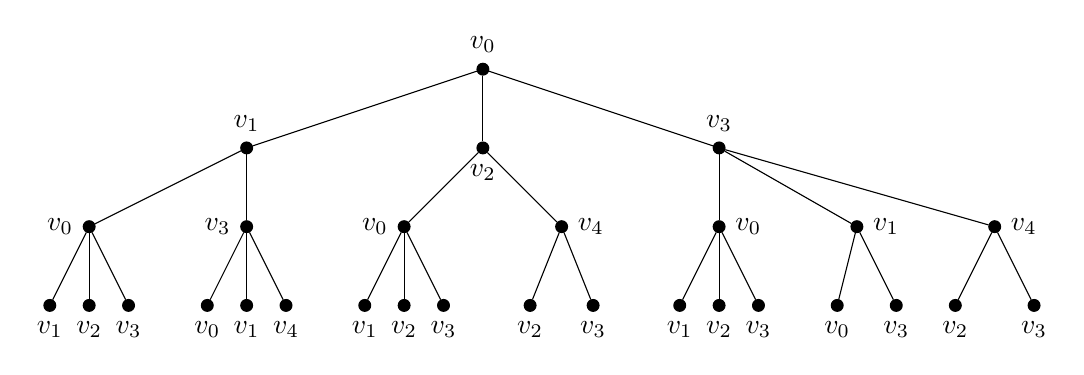
\begin{tikzpicture}

      \tikzset{enclosed/.style={draw, circle, inner sep=0pt, minimum size=.15cm, fill=black}}
%% Vertices
      	\node[enclosed, label={above: $v_0$}] (v0) at (3,6) {};
      	\node[enclosed, label={above: $v_1$}] (v1) at (0,5) {};
    		\node[enclosed, label={below: $v_2$}] (v2) at (3,5) {};
  	    \node[enclosed, label={above: $v_3$}] (v3) at (6,5) {};
     	\node[enclosed, label={left: $v_0$}] (v4) at (-2,4) {};
     	\node[enclosed, label={left: $v_3$}] (v5) at (0,4) {};
     	\node[enclosed, label={left: $v_0$}] (v6) at (2,4) {};
     	\node[enclosed, label={right: $v_4$}] (v7) at (4,4) {};
     	\node[enclosed, label={right: $v_0$}] (v8) at (6,4) {};
     	\node[enclosed, label={right: $v_1$}] (v9) at (7.75,4) {};
     	\node[enclosed, label={right: $v_4$}] (v10) at (9.5,4) {};
     	\node[enclosed, label={below: $v_1$}] (v11) at (-2.5,3) {};
      	\node[enclosed, label={below: $v_2$}] (v12) at (-2,3) {};
  	    \node[enclosed, label={below: $v_3$}] (v13) at (-1.5,3) {};
  	    \node[enclosed, label={below: $v_0$}] (v14) at (-0.5,3) {};
     	\node[enclosed, label={below: $v_1$}] (v15) at (0,3) {};
     	\node[enclosed, label={below: $v_4$}] (v16) at (0.5,3) {};
     	\node[enclosed, label={below: $v_1$}] (v17) at (1.5,3) {};
      	\node[enclosed, label={below: $v_2$}] (v18) at (2,3) {};
  	    \node[enclosed, label={below: $v_3$}] (v19) at (2.5,3) {};
  	    \node[enclosed, label={below: $v_2$}] (v20) at (3.6,3) {};
  	    \node[enclosed, label={below: $v_3$}] (v21) at (4.4,3) {};
  	    \node[enclosed, label={below: $v_1$}] (v22) at (5.5,3) {};
      	\node[enclosed, label={below: $v_2$}] (v23) at (6,3) {};
  	    \node[enclosed, label={below: $v_3$}] (v24) at (6.5,3) {};
  	    \node[enclosed, label={below: $v_0$}] (v25) at (7.5,3) {};
     	\node[enclosed, label={below: $v_3$}] (v26) at (8.25,3) {};
     	\node[enclosed, label={below: $v_2$}] (v27) at (9,3) {};
     	\node[enclosed, label={below: $v_3$}] (v28) at (10,3) {};
%Edges
		\path (v0) edge node[midway, sloped, above] {} (v1);
		\path (v0) edge node[midway, sloped, above] {} (v2);
		\path (v0) edge node[midway, above] {} (v3);
		\path (v1) edge node[near end, sloped, below] {} (v4);
		\path (v1) edge node[midway, below] {} (v5);
		\path (v2) edge node[near end, sloped, above] {} (v6);
		\path (v2) edge node[near end, sloped, above] {} (v7);
		\path (v3) edge node[near end, sloped, above] {} (v8);
		\path (v3) edge node[near end, sloped, above] {} (v9);
		\path (v3) edge node[near end, sloped, above] {} (v10);
		\path (v4) edge node[near end, sloped, above] {} (v11);
		\path (v4) edge node[near end, sloped, above] {} (v12);
		\path (v4) edge node[near end, sloped, above] {} (v13);
		\path (v5) edge node[near end, sloped, above] {} (v14);
		\path (v5) edge node[near end, sloped, above] {} (v15);
		\path (v5) edge node[near end, sloped, above] {} (v16);
		\path (v6) edge node[near end, sloped, above] {} (v17);
		\path (v6) edge node[near end, sloped, above] {} (v18);
		\path (v6) edge node[near end, sloped, above] {} (v19);
		\path (v7) edge node[near end, sloped, above] {} (v20);
		\path (v7) edge node[near end, sloped, above] {} (v21);
		\path (v8) edge node[near end, sloped, above] {} (v22);
		\path (v8) edge node[near end, sloped, above] {} (v23);
		\path (v8) edge node[near end, sloped, above] {} (v24);
		\path (v9) edge node[near end, sloped, above] {} (v25);
		\path (v9) edge node[near end, sloped, above] {} (v26);
		\path (v10) edge node[near end, sloped, above] {} (v27);
		\path (v10) edge node[near end, sloped, above] {} (v28);

	\end{tikzpicture}
	\caption{De mulige løsninger for veje med længde 3 fra $v_{0}$ til $v_{k}$}
	\label{fig.vaegtetopg}
\end{figure}

Antallet af veje fra $v_{0}$ til $v_{2}$ er 5 og antallet af veje fra $v_{0}$ til $v_{3}$ er 6. Vi kan derfor opstille
\textbf{$A^{4}$}$=b_{1i} \cdot a_{1j}+b_{2i} \cdot a_{2j}=5 \cdot 1+6 \cdot 1=11$
Her er $b_{1i}$ antallet af veje fra $v_{i}=v_{0}$ til vores første $v_{k}=v_{2}$ og $a_{1j}$ er antallet af kanter fra vores første $v_{k}=v_{2}$ til vores $v_{j}=v_{4}$. På samme måde optræder $b_{2i}$ og $a_{2j}$ for vores andet $v_{k}=v_{3}$. Der er altså 11 veje med længden 4 fra punktet $v_{0}$ til punktet $v_{4}$.

\input{incl/main/grafer/vægtede}